% Source: Lecture10.pdf, pages 1-7. The file has no lecture heading.
\lecture{10}
\subsection{Landau--Ginzburg approach to critical phenomena}

The Landau--Ginzburg (LG) approach to critical phenomena is based on an expansion of the
Helmholtz free energy around the critical temperature $T_c$. For definiteness, we will use
magnetic variables, and write the Helmholtz free energy as $A(T,M)$; the corresponding results for
a liquid--gas phase transition with $A(T,V)$ are obvious.

The LG approach is approximate, and the LG values of critical exponents differ from
experimentally measured values. But nevertheless, the LG approach is useful as a general way to
obtain critical exponents. Later, we will discuss the mean field theory (MFT) approach to phase
transitions. The LG values of critical exponents are equal to the MFT values. In both cases, these
approximations neglect fluctuations. LG theory does not make reference to the dimensionality of the
space or to the symmetry group of the Hamiltonian, $\Ham$. Since experimentally the critical
exponents do depend on the spatial dimension $d$ and the symmetry group of $\Ham$, it is clear that
the LG formalism is only approximate.

LG: write
\begin{equation}
  A(T,M) = \sum_{n=2}^\infty L_n(T)M^n,
\end{equation}
where $M$ = magnetization (e.g.\ $M = \ev{\sigma}$ for the Ising model). (We can drop the $n = 0$
term for our calculations here involving derivatives with respect to $M$.) Since $A(T,M)$ does not
depend on $\sgn(M)$, only even $n$ contribute to this sum. For a continuous phase transition, only
the lowest-order terms in the expansion are important near $T_c$, where $M$ is small. For a
bicritical point we can keep just the $M^2$ and $M^4$ terms:
\begin{equation}
  A(T,M) = L_2(T)M^2 + L_4(T)M^4 + \Order(M^6).
\end{equation}
Next, expand the $L_n(T)$, $n = 2,4$:
\begin{equation}
  L_n(T) = \sum_{k=0}^\infty\ell_{n,k}(T-T_c)^k .
\end{equation}
To fit the dependence of $M$ on $T$, set $\ell_{2,0} = 0$. For boundedness of the Helmholtz energy
as a function of $M$, set $\ell_{4,0}>0$. Then, to leading order, near $T = T_c$,
\begin{equation}
  A(T,M) = \ell_{2,1}(T-T_c)M^2 + \ell_{4,0}M^4 + \ldots
\end{equation}
(higher orders in powers of $M^2$ and powers of $T-T_c$); set $\ell_{2,1}>0$ to agree with the
physical behavior of $M$.

\begin{diagram}
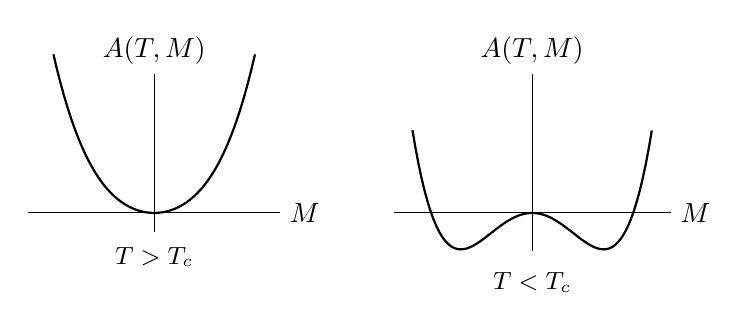
\begin{tikzpicture}[scale=0.8]
  \draw (-2,0) -- (2,0) node[right] {$M$}; \draw (0,-0.3) -- (0,2.2) node[above] {$A(T,M)$};
  \draw[thick,domain=-1.6:1.6,samples=60] plot (\x,{0.6*\x*\x+0.15*\x*\x*\x*\x});
  \node[font=\small] at (0,-0.7) {$T>T_c$};
  \begin{scope}[xshift=6cm]
  \draw (-2.2,0) -- (2.2,0) node[right] {$M$}; \draw (0,-0.6) -- (0,2.2) node[above] {$A(T,M)$};
  \draw[thick,domain=-1.9:1.9,samples=80] plot (\x,{-0.9*\x*\x+0.35*\x*\x*\x*\x});
  \node[font=\small] at (0,-1.1) {$T<T_c$};
  \end{scope}
\end{tikzpicture}
\diagramcaption{Graphically: for $T>T_c$ the minimum of the Helmholtz free energy is at $M = 0$,
so there is no magnetization. For $T<T_c$ the minima of $A(T,M)$ are at nonzero $\pm M$,
indicating nonzero magnetization.}
\end{diagram}

This results because $L_2(T)$ reverses sign as $T$ passes through $T_c$.

Calculate the position of the minimum of $A$: this occurs where $\partial A/\partial M = 0$ with
$\partial^2A/\partial M^2>0$:
\begin{equation}
  \pder{A}{M} = 2\ell_{2,1}(T-T_c)M + 4\ell_{4,0}M^3 = 2M\left[\ell_{2,1}(T-T_c) + 2\ell_{4,0}M^2\right].
\end{equation}
For $T>T_c$, the minimum of $A$ is at $M = 0$. For $T<T_c$, the minimum of $A$ is at
\begin{equation}
  M = \pm\left[\frac{\ell_{2,1}(T_c-T)}{2\ell_{4,0}}\right]^{1/2}.
\end{equation}
The sign of $\partial^2A/\partial M^2$ at these points:
\begin{align}
  \frac{\partial^2A}{\partial M^2} &= 2\ell_{2,1}(T-T_c) + 12\ell_{4,0}M^2
    = 2\ell_{2,1}(T-T_c) + 12\ell_{4,0}\left(-\frac{\ell_{2,1}(T-T_c)}{2\ell_{4,0}}\right)\nonumber\\
  &= 2\ell_{2,1}(T-T_c) - 6\ell_{2,1}(T-T_c) = 4\ell_{2,1}(T_c-T)>0\quad\text{for } T<T_c
\end{align}
(and $=2\ell_{2,1}(T-T_c)$ for $T>T_c$, where $M = 0$). This shows that these are minima of $A$,
which is clear from the graphs.

Recall the definition of the critical exponent $\beta$: $M\propto(T_c-T)^\beta$ as
$T_c-T\to 0^+$, i.e.\ $\ln M = \beta\ln(T_c-T)$,
\begin{equation}
  \beta = \lim_{T\to T_c^-}\frac{\ln M}{\ln(T_c-T)}.
\end{equation}
From our solution for $M$ above, we find
\begin{equation}
  \text{LG:}\quad\boxed{\beta = \frac{1}{2}}.
\end{equation}

Next, calculate the magnetic susceptibility $\chi = \partial M/\partial H$ as $T\to T_c$ and the
corresponding critical exponents:
\begin{equation}
  \chi\propto
  \begin{cases}
    (T-T_c)^{-\gamma} & \text{as } T\to T_c^+\\
    (T_c-T)^{-\gamma'} & \text{as } T\to T_c^- .
  \end{cases}
\end{equation}
Recall $\dd A(T,M) = -S\dd T + H\dd M$, so
\begin{equation}
  H = \left(\pder{A}{M}\right)_T;\qquad \pder{H}{M} = \left(\frac{\partial^2A}{\partial M^2}\right)_T,
  \qquad\text{i.e.}\quad \chi = \left(\pder{M}{H}\right) = \left[\frac{\partial^2A}{\partial M^2}\right]^{-1}.
\end{equation}
Now we calculated $(\partial^2A/\partial M^2)_T$ above: for $T>T_c$, the minimum of $A$ is at
$M = 0$, where $\partial^2A/\partial M^2 = 2\ell_{2,1}(T-T_c)>0$. So as $T\to T_c^+$,
\begin{equation}
  \chi\simeq\frac{1}{2\ell_{2,1}(T-T_c)},\qquad\text{so}\quad\boxed{\gamma = 1}.
\end{equation}
For $T<T_c$, $\partial^2A/\partial M^2 = 4\ell_{2,1}(T_c-T)$ at the minimum of $A$
$\Rightarrow\chi = [4\ell_{2,1}(T_c-T)]^{-1}\Rightarrow\gamma' = 1$.

So the LG approach yields $\beta = 1/2$ and $\gamma = \gamma' = 1$. (Note that the critical
amplitudes for $\chi$ for $T>T_c$ and $T<T_c$ are different:
\begin{equation}
  \chi\sim
  \begin{cases}
    \dfrac{1}{2\ell_{2,1}(T-T_c)} & \text{as } T-T_c\to 0^+\\[8pt]
    \dfrac{1}{4\ell_{2,1}(T_c-T)} & \text{as } T-T_c\to 0^- .)
  \end{cases}
\end{equation}

Next, calculate the LG value for the critical exponent describing the critical isotherm,
$|M|^\delta\sgn(M) = H$ at $T_c$. Take $H>0$, so $M^\delta = H$, i.e.\ $M = H^{1/\delta}$ at $T_c$.
Now from $\dd A(T,M) = -S\dd T + H\dd M$, with $H = (\partial A/\partial M)_T$, recall
$(\partial A/\partial M)_T = 2\ell_{2,1}(T-T_c)M + 4\ell_{4,0}M^3$. Set $T = T_c$; then
\begin{equation}
  \left(\pder{A}{M}\right)_{T=T_c} = 4\ell_{4,0}M^3 = H,\qquad\text{so}\quad
  \text{LG:}\ \boxed{\delta = 3}.
\end{equation}

\begin{diagram}
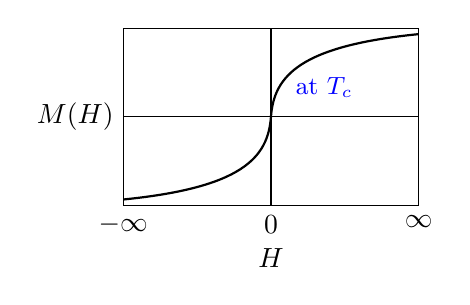
\begin{tikzpicture}[scale=0.75]
  \draw (0,0) rectangle (5,3); \draw (0,1.5) -- (5,1.5); \draw (2.5,0) -- (2.5,3);
  \draw[thick] (0,0.1) .. controls (2,0.3) and (2.45,0.8) .. (2.5,1.5) .. controls (2.55,2.2) and (3,2.7) .. (5,2.9);
  \node[left] at (0,1.5) {$M(H)$};
  \node[below] at (0,0) {$-\infty$}; \node[below] at (2.5,0) {$0$}; \node[below] at (5,0) {$\infty$};
  \node[below=12pt] at (2.5,0) {$H$};
  \node[blue,font=\small] at (3.4,2.0) {at $T_c$};
\end{tikzpicture}
\diagramcaption{The critical isotherm.}
\end{diagram}

The approximate nature of the Landau--Ginzburg formalism is clear from the fact that it is based on
an expansion of the Helmholtz free energy $A(T,M)$ as a function of $M$ and $T$, about $T = T_c$,
$M = 0$. This would be justified if $A(T,M)$ were analytic at this point, but it is not, as is
evident from $M(T)$ and $\chi(T)$.

\begin{diagram}
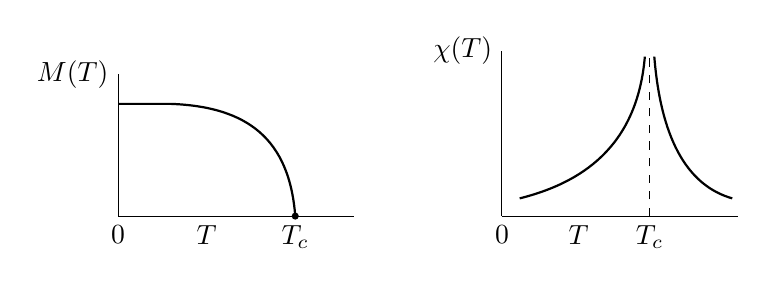
\begin{tikzpicture}[scale=0.75]
  \draw (0,0) -- (4,0); \draw (0,0) -- (0,2.4) node[left] {$M(T)$};
  \draw[thick] (0,1.9) -- (0.9,1.9) .. controls (2.2,1.85) and (2.9,1.3) .. (3,0);
  \fill (3,0) circle (0.06);
  \node[below] at (0,0) {$0$}; \node[below] at (1.5,0) {$T$}; \node[below] at (3,0) {$T_c$};
  \begin{scope}[xshift=6.5cm]
  \draw (0,0) -- (4,0); \draw (0,0) -- (0,2.8) node[left] {$\chi(T)$};
  \draw[dashed] (2.5,0) -- (2.5,2.8);
  \draw[thick] (0.3,0.3) .. controls (1.5,0.6) and (2.3,1.3) .. (2.42,2.7);
  \draw[thick] (2.58,2.7) .. controls (2.7,1.2) and (3.2,0.5) .. (3.9,0.3);
  \node[below] at (0,0) {$0$}; \node[below] at (1.3,0) {$T$}; \node[below] at (2.5,0) {$T_c$};
  \end{scope}
\end{tikzpicture}
\diagramcaption{The magnetization and susceptibility are nonanalytic at $T_c$.}
\end{diagram}

Nevertheless, the LG formalism provides a useful approximate approach to critical behavior.

\subsection{Mean field theory approach to phase transitions}\label{sec:mft}

For definiteness, we discuss MFT using the simplest spin model as an illustration, namely the Ising
model. Then we generalize to other spin models.
\begin{equation}
  Z = \sum_{\{\sigma_i\}}e^{-\beta\Ham},\qquad
  \Ham = -J\sum_{e_{ij}}\sigma_i\sigma_j - H\sum_i\sigma_i,\qquad\beta = \frac{1}{\kB T},
\end{equation}
\begin{equation}
  Z = \sum_{\{\sigma_i\}}e^{K\sum_{e_{ij}}\sigma_i\sigma_j + h\sum_i\sigma_i},
  \qquad\text{where, as before,}\quad K\equiv\beta J,\ h\equiv\beta H .
\end{equation}
What makes the calculation of $Z$ and $f = \lim_{N\to\infty}(1/N)\ln Z$ difficult is the coupled,
many-body (actually infinite in the $N\to\infty$ limit) nature of the problem. MFT simplifies the
problem drastically by approximating the coupled many-body problem by a 1-body problem, assuming
that a given spin $\sigma_0$ interacts with a mean (= average) magnetic field due to all of the other
spins. So the actual $\Ham$ is replaced by
\begin{equation}
  \Ham_{\text{MFT}} = -J\sum_{\text{n.n.}\,i}\sigma_0\sigma_i - H\sigma_0,\qquad\text{i.e.}\quad
  -\beta\Ham_{\text{MFT}} = K\sum_{\text{n.n.}\,i}\sigma_0\sigma_i + h\sigma_0,
\end{equation}
where $\sigma_i = \ev{\sigma_i}$, the mean magnetization $\bar M$, and n.n.\ $i$ = nearest-neighbor
sites $i$ (adjacent vertices in the terminology of graph theory). The physical application is to the
model on a regular lattice with coordination number = vertex degree $\Delta$, with
$\ev{\sigma_i} = \bar M$. So
\begin{equation}
  -\beta\Ham_{\text{MFT}} = K\Delta\sigma_0\bar M + h\sigma_0 = (K\Delta\bar M + h)\sigma_0,
\end{equation}
so for the single site, denoted 0,
\begin{equation}
  Z_{ss,\text{MFT}} = \sum_{\sigma_0=\pm1}e^{(K\Delta\bar M+h)\sigma_0}
  = e^{K\Delta\bar M+h} + e^{-(K\Delta\bar M+h)} = 2\cosh(K\Delta\bar M+h),
\end{equation}
and $Z_{\text{MFT}} = (Z_{ss,\text{MFT}})^N$,
\begin{equation}
  f_{\text{MFT}} = \lim_{N\to\infty}\frac{1}{N}\ln Z_{\text{MFT}} = \ln[Z_{ss,\text{MFT}}]
  = \ln[2\cosh(K\Delta\bar M+h)].
\end{equation}
The Gibbs free energy is $G_{\text{MFT}}(T,H) = -\kB Tf_{\text{MFT}}$, and
\begin{equation}
  \bar M = \pder{f}{h} = \tanh(K\Delta\bar M + h)\quad\text{in MFT}.
\end{equation}
The spontaneous magnetization is
\begin{equation}
  \bar M_{sp} = \lim_{H\to 0}\bar M = \tanh(K\Delta\bar M_{sp}).
\end{equation}
At high temperature, $\beta\to 0$, so the only solution is $\bar M_{sp} = 0$. As $T$ decreases
($\beta$ increases) a nonzero solution first occurs (i.e.\ $\bar M_{sp}$ increases from zero) when,
expanding the tanh, $\bar M_{sp} = K\Delta\bar M_{sp}$, i.e.\ at $K\Delta = 1$,
\begin{equation}
  K_{c,\text{MFT}} = \frac{1}{\Delta}.
\end{equation}
(Here we used the Taylor series expansion $\tanh x\simeq x + \Order(x^3)$ for $x\to 0$.) So the
critical temperature in the MFT approximation is $K_{c,\text{MFT}} = 1/\Delta$, i.e.\
$\beta_{c,\text{MFT}} = 1/(J\Delta) = 1/(\kB T_{c,\text{MFT}})$, so
\begin{equation}
  T_{c,\text{MFT}} = \frac{J\Delta}{\kB}.
\end{equation}
Note the dependence on the lattice coordination number, but no explicit dependence on lattice
dimensionality. Thus the MFT prediction for $T_c$ for the Ising model on the triangular lattice,
which is 2-dimensional, is the same as the prediction for $T_c$ for the Ising model on the simple
cubic lattice, which is 3-dimensional, since both have the same coordination number, $\Delta = 6$.
In reality, these $T_c$ values are not equal. This shows one deficiency in MFT.

Furthermore, MFT neglects fluctuations, which tend to disorder the spins, so one must actually make
$T$ \emph{lower} than the MFT prediction, $(T_c)_{\text{MFT}}$, in order for the phase transition to
occur and for a nonzero spontaneous magnetization (LRO). For example, we will later derive
$K_{c,sq}$, the critical $K_c$ for the Ising model on the square lattice. This is
\begin{equation}
  K_{c,sq} = \frac{1}{2}\ln(1+\sqrt2) = 0.4407,
\end{equation}
and, with $K = \beta J = J/(\kB T)$, this means that
\begin{equation}
  \kB T_{c,sq} = \frac{2J}{\ln(1+\sqrt2)} = 2.269\,J .
\end{equation}
Compare with $K_{c,\text{MFT}} = 1/\Delta_{sq} = 1/4 = J/(\kB T_{c,\text{MFT}})$
$\Rightarrow\kB T_{c,\text{MFT}} = 4J$. So
\begin{equation}
  \frac{T_{c,sq}}{T_{c,\text{MFT}}} = \frac{K_{c,\text{MFT}}}{K_{c,sq}}
  = \frac{1/4}{(1/2)\ln(1+\sqrt2)} = \frac{1}{2\ln(1+\sqrt2)} = 0.5673,
\end{equation}
which is $<1$, for the reason given above: the neglect of disordering fluctuations in MFT.

\subsubsection*{Critical exponents in MFT}

Use $\bar M_{sp} = \tanh(K\Delta\bar M_{sp})$ and the expansion
$\tanh x = x - (1/3)x^3 + \Order(x^5)$ as $x\to 0$, so
\begin{equation}
  \bar M_{sp} = K\Delta\bar M_{sp} - \frac{1}{3}(K\Delta\bar M_{sp})^3 + \Order\left((K\Delta\bar M_{sp})^5\right)
\end{equation}
as $T\to T_c^-$, and hence $\bar M_{sp}\to 0$. For $T<T_c$, divide both sides by $\bar M_{sp}$, which
is nonzero:
\begin{align}
  &\Rightarrow 1 = K\Delta - \frac{1}{3}(K\Delta)^3\bar M_{sp}^2 + \Order\left((K\Delta)^5\bar M_{sp}^4\right)
    = K\Delta\left[1-\frac{1}{3}(K\Delta)^2\bar M_{sp}^2+\ldots\right]\nonumber\\
  &\Rightarrow\frac{1}{K\Delta} = 1-\frac{1}{3}(K\Delta)^2\bar M_{sp}^2+\ldots
  \ \Rightarrow\ \bar M_{sp}^2 = \frac{3}{(K\Delta)^2}\left[1-\frac{1}{K\Delta}\right]
  \quad\text{as } T\to T_c^-,
\end{align}
where the $\Order((K\Delta)^5\bar M_{sp}^4)$ term is negligible as $T\to T_c^-$. Then
\begin{equation}
  \bar M_{sp}^2 = \frac{3}{(K\Delta)^2}\left[1-\frac{1}{K\Delta}\right]
  = \frac{3}{(K\Delta)^2}\left[1-\frac{K_c}{K}\right] = \frac{3}{K^3\Delta^2}(K-K_c).
\end{equation}
Now $K-K_c = J(\beta-\beta_c) = (J/\kB)\left(1/T-1/T_c\right) = (J/(\kB TT_c))(T_c-T)$,
so
\begin{equation}
  \bar M_{sp}^2 = \left(\frac{3}{K_c^3\Delta^2}\right)\underbrace{\left(\frac{J}{\kB T_c}\right)}_{K_c}\left(\frac{T_c-T}{T_c}\right)
  = \frac{3}{(K_c\Delta)^2}\left(\frac{T_c-T}{T_c}\right),
\end{equation}
where $3/(K_c\Delta)^2$ is a constant. So $\bar M_{sp}\propto(T_c-T)^{1/2}$ as $T\to T_c^-$, so the
critical exponent is
\begin{equation}
  \boxed{\beta = \frac{1}{2}\ \text{in MFT}}.
\end{equation}

Next, calculate the critical behavior of $\chi$ and the associated exponents $\gamma$, $\gamma'$:
use the basic MFT equation $\bar M = \tanh(K\Delta\bar M + h)$. Now expand for $T$ near $T_c$, using
$\tanh x = x - x^3/3 + \Order(x^5)$ for small $x$, and use
$\bar\chi = \partial M/\partial H = \beta\partial M/\partial h$, so $\beta^{-1}\bar\chi = \partial M/\partial h$:
\begin{equation}
  \bar M = (K\Delta\bar M + h) - \frac{1}{3}(K\Delta\bar M+h)^3+\ldots,\qquad
  (1-K\Delta)\bar M = h - \frac{1}{3}(K\Delta\bar M+h)^3+\ldots
\end{equation}
Let $K\Delta\equiv\kappa$. Then
\begin{equation}
  \Rightarrow\ \bar M = \frac{h}{(1-K\Delta)} - \frac{1}{3(1-K\Delta)}\left[(\kappa\bar M)^3 + 3(\kappa\bar M)^2h + 3(\kappa\bar M)h^2 + h^3\right]+\ldots
\end{equation}
The first term is the leading-order behavior as $T\to T_c$, so $\partial \bar M/\partial h = 1/(1-K\Delta)$:
\begin{equation}
  \beta^{-1}\bar\chi = \frac{1}{1-K\Delta} = \frac{1}{1-K/K_c}\propto\frac{1}{K_c-K}\propto\frac{1}{T-T_c},
\end{equation}
so $\gamma = 1$; similarly, $\gamma' = 1$. The other terms are negligible as $T\to T_c$ (HW).
Similarly, the critical exponent for the critical isotherm is $\delta = 3$.

\subsubsection*{Comparison of \texorpdfstring{$T_{c,\text{MFT}}$}{Tc,MFT} with actual values}

It is of interest to compare the MFT prediction for $T_c$ with the actual values of $T_c$ for 3D
lattices, extending our previous comparison for the square lattice (2D). Consider the simple cubic
(sc) lattice. Analysis of high-$T$ series expansions $\Rightarrow\tanh(K_{c,sc})\simeq 0.21813$
$\Rightarrow K_{c,sc}\simeq 0.22169$, and
\begin{equation}
  \frac{T_{c,sc}}{T_{c,\text{MFT},sc}} = \frac{K_{c,\text{MFT},sc}}{K_{c,sc}} = \frac{1/6}{0.2217}\simeq 0.752 .
\end{equation}
From this comparison, we see that as the dimension (coordination number) increases, the MFT
prediction for $T_c$ becomes more accurate; this ratio was 0.567 for the square lattice.

Let us give another comparison, for the body-centered cubic (bcc) lattice; see the picture in
Figure~\ref{fig:cubic}; $\Delta = 8$ for the bcc lattice. Analysis of high-temperature series
expansions gives $K_{c,bcc} = 0.157407$, so
\begin{equation}
  \frac{T_{c,bcc}}{(T_c)_{\text{MFT},bcc}} = \frac{K_{c,\text{MFT},bcc}}{K_{c,bcc}} = \frac{1/8}{0.157407}\simeq 0.7941 .
\end{equation}
Summary of these comparisons:
\begin{center}
\begin{tabular}{lcc}
  lattice & $T_c/T_{c,\text{MFT}}$ & $\Delta$\\ \hline
  sq & 0.57 & 4\\
  sc & 0.75 & 6\\
  bcc & 0.79 & 8
\end{tabular}
\end{center}
This shows a trend, namely that as $\Delta$ increases, the MFT prediction for $T_c$ becomes more
accurate. An early review is by C.~Domb in the C.~Domb and M.~Green series entitled \emph{Phase
Transitions and Critical Phenomena}; see vol.~3.
